\documentclass[Royal,times,sageh]{sagej}

\usepackage{moreverb,url,natbib, multirow, tabularx}
\usepackage[colorlinks,bookmarksopen,bookmarksnumbered,citecolor=red,urlcolor=red]{hyperref}



\usepackage{hyperref}
\usepackage[utf8]{inputenc}
\usepackage{dcolumn}
\def\tightlist{}
\newcommand{\beginappendix}{\setcounter{table}{0} \renewcommand{\thetable}{A\arabic{table}} \setcounter{figure}{0} \renewcommand{\thefigure}{A\arabic{figure}}}


\begin{document}

\title{Working from home and digital divides: resilience in the time of a
pandemic}

\runninghead{}

\author{A. Uthor*\affilnum{1,2}, O. Tro\affilnum{2}, O. Vriga\affilnum{3}}

\affiliation{\affilnum{1}{Department of Incredible Research, University A, City A, Country A}\\\affilnum{2}{Department of Applied Things, University B, City B, Country B}\\\affilnum{3}{Very Important Stuff Committee, Institute C, City C, Country C}}

\corrauth{Corresponding author name, This is sample corresponding address.}

\email{\href{mailto:correspondingauthor@protonmail.com}{\nolinkurl{correspondingauthor@protonmail.com}}}

\begin{abstract}
This paper offers a new perspective on telecommuting from the viewpoint
of the complex web of digital divides. Using the UK as a case study,
this paper studies how the quality and reliability of internet service,
as reflected in \emph{experienced} vis-à-vis \emph{advertised} upload
internet speeds during the spring 2020 lockdown, may reinforce or
redress the spatial and social dimensions of digital divisions. Fast,
reliable internet connections are necessary for the population to be
able to work from home. Although not every place hosts individuals in
occupations which allow for telecommuting nor with the necessary skills
to effectively use the internet to telecommute, we raise the issue that
without good internet connectivity, these places would struggle more to
achieve economic resilience in a period like the current pandemic. We
employ data on individual broadband speed tests and state-of-the-art
time-series clustering methods to create clusters of UK local
authorities with similar temporal signatures of experienced internet
speeds. We then associate these clusters of local authorities with their
socioeconomic and geographic characteristics to explore how they overlap
with or diverge from the existing economic and digital geography of the
UK. Our analysis enables us to better understand how the spatial and
social distribution of both occupations and online accessibility
intersect to enable or hinder the practice of telecommuting at a time of
extreme demand.
\end{abstract}

\keywords{covid; internet; working from home; broadband speed; time-series
clusters;}

\maketitle

\hypertarget{sec:1}{%
\section{Introduction}\label{sec:1}}

During the pandemic, working from home using digital technologies,
whether partially or exclusively, was transformed from a niche means of
accessing work, albeit one that had been on a slow, upward trend, to a
widespread way of life in many countries. The ability to work from home
or telecommute meant millions retained their jobs and, to a varying
extent, maintained productivity during periods of strict lockdowns
around the world. However, this ability has not been evenly distributed
socially or spatially, creating new intersections of economic and
digital divisions. On one side are those who can work from home,
supported by digital technologies, and have thus been able to enjoy both
economic resilience and greater personal safety. On the other side,
previously employed individuals have been forced to accept furlough or
redundancy packages unless they are part of the cadre of essential
workers, who are potentially at high risk of infection. Whilst the basis
for this pandemic-generated divide has been viewed as mainly
occupational, here we consider whether it is also technological and,
consequently, geographical.

Using the UK as a case study, this paper aims to understand how the
quality and reliability of internet service, as reflected in
\emph{experienced} internet speeds during the spring 2020 lockdown, may
reinforce or redress the spatial and social dimensions of digital
divisions. We employ volunteered geographic data on individual broadband
speed tests and state-of-the-art time-series clustering methods to
create clusters of UK local authorities with similar temporal signatures
of experienced internet speeds. We then associate these clusters of
local authorities with their socioeconomic and geographic
characteristics to explore how they overlap with or diverge from the
existing economic and digital geography of the UK. Our analysis enables
us to better understand how the spatial and social distribution of both
occupations and online accessibility intersect to enable or hinder the
practice of telecommuting at a time of extreme demand. We also consider
what lessons can be learned from this time for a future where
telecommuting is likely to remain a more common means of accessing work,
at least in comparison to the pre-Covid era, and broadband services and
infrastructure must be fit for purpose.

The capability to work from home has previously been studied from the
perspective of whether work tasks in a given occupation both can be and
are allowed to be performed using digital technologies independently of
location or co-location with colleagues, including supervisors
\citep{allen2015effective, singh2013modeling}. However, successful
telecommuting also requires that the quality and reliability of digital
services, particularly home internet connection speeds, enable the
completion of work tasks with a minimum of delay or interruption. Prior
to the pandemic, the performance of broadband services with respect to
telecommuters was never tested at scale, as working from home and
connecting to colleagues and workplace resources via the internet was
the purview of a small minority of workers. Instead, leisure use in the
evening, when video streaming services are at their peak, has been used
to benchmark broadband performance and service delivery by different
Internet Service Providers (ISPs) \citep{ofcom2017}.

Yet the shift towards telecommuting during various stages of lockdown
around the world has been drastic and there are speculations that
post-Covid, the tendency to work from home will be much higher, raising
questions around whether internet services can accommodate the increased
demand. For example, \(47\)\% of people in employment in the UK worked
solely from home in April \(2020\), whilst the same figure only reached
\(5\)\% the year before \citep{ons2020, ons2020lm2019}. A back of the
envelope calculation suggests that up to 40\% of the labour force could
work from home on an ongoing basis \citep{batty2020editorial}. Similar
figures have been reported for other countries
\citep{felstead2020homeworking}. Approximately \(37\)\% of the European
workforce worked from home in April \(2020\) with countries like Finland
reaching \(60\)\% \citep{eurofound2020}. In the US, almost half of the
working population worked from home during the same period because of
the pandemic \citep{brynjolfsson2020covid}, and a recent estimate
indicated that \(37\)\% of all jobs in the US can be permanently
performed entirely from home \citep{NBERw26948}. None of these changes
could have happened in the absence of reliable information and
communication technology (ICT) infrastructure -- both in terms of
software and hardware. But while software innovations are easily
diffused across space and society\footnote{See for example the huge
  success of videoconferencing apps such as Zoom \citep{marks2020zoom}.},
the same does not apply for ICT hardware infrastructure such as internet
broadband connectivity.

The literature describes first level digital divides in terms of the
availability and quality of internet connectivity, such as that manifest
in different geographies in the UK
\citep{riddlesden2014broadband, philip2017digital}. Second level digital
divides consider the presence or lack of the necessary skills to
effectively utilise digital technologies and the internet
\citep{blank2014dimensions, van2011internet}. The third level focuses on
the heterogenous returns of internet usage among different socioeconomic
groups and, consequently, how digital technologies can assist in
bridging or further enhancing existing socioeconomic divides.
\citep{stern2009levels, van2014digital, van2015third}. The capability to
telecommute is related to all three levels of digital divides, but more
importantly leads to differentiated outcomes regarding the economic
resilience of people and places to overcome a systemic shock such as the
current pandemic.

As the quality of internet infrastructure and services, as well as the
concentration of different occupations are spatially dependent and
clustered in space, our approach offers a framework for understanding
the impact of and interactions between digital divisions geographically
and socioeconomically. By asking how resilient broadband speeds, and
particularly upload speeds, are experienced in different parts of the UK
during a time of extreme demand, we interrogate which places benefit
from the greater economic resilience digital technologies can offer. The
structure of this paper is as follows. First we review the literature on
telecommuting and digital divides to better understand their structural
and spatial development pre-pandemic, and thus their importance to the
economic resilience of different places. We then describe our data and
methodology. Our results section first offers a classification of how
internet services vary across clusters of UK local authorities and then
assesses whether these clusters replicate or repudiate other
socio-economic and geographic patterns of economic resilience. We
conclude with a discussion of the insights we have gained from our new
perspective on digital divisions.

\hypertarget{sec:2}{%
\section{Literature review}\label{sec:2}}

\hypertarget{sec:2.1}{%
\subsection{From telecommuting to \#WFH}\label{sec:2.1}}

In this analysis, the terms `telecommuting' and `working from
home\footnote{See also the popular social media hashtag \#WFM}' are used
interchangeably, as most remote labour during the Covid-19 crisis was
carried out in the homes of individual employees rather than any other
location \citep{eurofound2020}. However, it should be noted that
previous research has explored how telecommuting can occur in other
places, including satellite offices or on public transport
\citep{felstead2012rapid, siha2006telecommuting}. Previous research has
also used a variety of definitions to measure the level of telecommuting
within different workforces, distinguishing, for example, between those
directly employed, indirectly employed, self-employed, full-time or
part-time, and those who use digital technologies to work remotely
full-days or part-days
\citep{allen2015effective, bailey2002review, haddad2009examination}. No
matter the definition, the option and capability to telecommute or work
from home has never been equally distributed spatially or
socio-economically any more than different industries and employment
opportunities have. For example, studies from the United States, the
Netherlands, and the UK found that telecommuters are most likely to hold
professional, managerial, and technical occupations where the workforce
is better educated and wealthier, and that there is suppressed demand
among women and part-time workers
\citep{headicar2016move, peters2004employees, singh2013modeling}.

Opportunities for working from home during the current pandemic have
likewise not been equally spread across the workforce.
\citet{NBERw26948} indicated that in the US, managers, educators, as
well as those working in computer-related occupations, finance, and law
can easily work from home, and that occupations with opportunities to
telecommute are associated with higher earnings. This is not the case
for the workforce occupied in more spatially fixed occupations, from
farming, construction and manufacturing to hospitality and care
services. In the US, these occupations tend to be lower-income,
non-white, without a university degree, live in rental accommodation and
lack health insurance \citep{NBERw27085}. Similar trends can be observed
for other countries. For example, \(75\)\% of workers with tertiary
education worked from home in Europe during spring \(2020\), whilst only
\(34\)\% of workers with secondary education and \(14\)\% of those
primary education did so \citep{eurofound2020}.

\hypertarget{sec:2.2}{%
\subsection{Digital divides and economic resilience}\label{sec:2.2}}

Our understanding of telecommuting as a product of enabled occupations
can be described as a manifestation of the third level digital divide,
as those who are able to use digital technologies to work from home
benefit from a high rate of return on their use of the internet in terms
of autonomy, flexibility, and time saved from commuting
\citep{peters2004employees, siha2006telecommuting, singh2013modeling}.
These returns have been even greater during the Covid-19 crisis, when
those with the capability to telecommute also have the ability to
maintain their employment whilst protecting their health. However, the
success of these arrangements has been dependent upon the first level
digital divide, which is associated with access to and quality of
internet connectivity. \citet{SALEMINK2017360} provides a systematic
review of the pre-pandemic, first level digital divide in infrastructure
quality between urban and rural areas in various advanced economies.
Rural areas, predictably, fare worse. Yet whether this variation in
infrastructure quality affects the spatial footprint of telecommuting
has not previously been discussed, in part because telecommuting has not
previously been the cause of greatest demand and pressure on internet
services.

There are indications that those who purchase high speed connections
consume more data of all sorts and use their connections for a variety
of purposes \citep{hauge2011consumer}. There is also a correlation
between access to internet services and a reduction in household
transport spend \citep{bris2017ict}. Independently of whether the
additional internet use and reduced travel is because of increased
telecommuting, these studies suggest that better internet services
enable households to make savings and efficiencies, an example of the
first level digital divide reinforcing the third level.

The extreme demand during the pandemic provides a new opportunity to
understand how infrastructure accessibility, quality, and reliability
affects telecommuting, particularly in light of the high volumes of
bandwidth-intensive video conferencing required in order to avoid the
face-to-face contact that could increase the spread of infection. We
seek to answer how internet service resilience contributes to or reduces
economic resilience when the latter is dependent upon the capability to
work from home. We also aim to improve our understanding of the impact
of first level digital division on telecommuting, and whether this
results in much more fundamental third level digital division than has
previously been perceived.

Furthermore, these multi-layered digital divides intersect with material
divides and the economic geography of the UK. Following the regional
economic resilience literature, which underlines the differentiated
capacity of cities and regions to escape or recover from economic crises
\citep{martin2012regional, kitsos2018economic}, different places have
different industrial and occupational profiles, and these affect the
aggregated potential capacity of places for telecommuting. Such profiles
are associated with longstanding inequalities in the UK and their
spatial representation as a North-South divide
\citep{martin_north_south}. Various studies have illustrated severe
inequalities between the north and the south regions of England
regarding, for example, skills and human capital, unemployment,
productivity and prosperity
\citep{lee2014grim, mccann2020perceptions, dorling2018peak}. Some
scholars have even argued that the UK suffers some of the highest level
of interregional inequalities in the global north
\citep{gal2018reducing, mccann2016uk}. Not only are all three levels of
digital divides associated with or shaped by the geography of the UK,
but the intersection of the digital and material divides affects the
capacity of places to overcome some of the economic effects of the
Covid-19 pandemic. Importantly, this is the first time that digital
technologies became an essential tool for economic resilience for such a
great part of the population.

\hypertarget{sec:3}{%
\section{Methods and data}\label{sec:3}}

\hypertarget{sec:3.1}{%
\subsection{Time-Series clustering}\label{sec:3.1}}

First we identified our methodological framework as cluster analysis,
which can be defined within the modern machine learning framework as an
unsupervised learning task, partitioning unlabelled observations into
homogeneous groups known as clusters \citep{montero2014tsclust}. The key
idea is that observations within clusters tend to be more similar than
observations between clusters. Clustering is particularly useful for
exploratory studies as it identifies structures within the data
\citep{aghabozorgi2015time}. Therefore, cluster analysis is a widely
used in geography \citep{gordon1977classification, everitt1974cluster}.
For instance, clustering methods are the basis of
\emph{geodemographics}, a research domain which aims to create small
area indicators or typologies of neighbourhoods based on diverse
variables \citep{SINGLETON2009289, harris2005geodemographics}. They have
also been employed to solve \emph{regionalisation} problems
\citep{niesterowicz2016}. Common characteristics of these studies are
the cross-sectional nature of the data they employ. Indeed, most
clustering problems in geography deal with observations that are fixed
in time. However, for this paper we are interested in internet speeds,
which vary over time and, therefore, we create clusters of local
authorities in the UK with similar temporal signatures of experienced
internet speeds.

To do so, we employ time-series clustering methods, which have been
developed to deal with clustering problems linked to, for instance,
stock or other financial data, economic, governmental or medical data as
well as machine monitoring
\citep{aggarwal2013time, aggarwal2001surprising, hyndman2015large, WARRENLIAO20051857}.
The main challenge -- and also the difference with cross-sectional
clustering problems -- is data dimensionality given the multiplicity of
data points for every individual object, local authorities in our case,
included in the data set. Time-series are dynamic data as the value of
the observations change as a function of time
\citep{aghabozorgi2015time}. This high dimensionality leads to (i)
computational and algorithmic challenges regarding handling these data
and building algorithms to perform clustering over long time-series, and
(ii) open questions regarding the choice of similarity measures in order
to cluster similar times-series objects together considering the whole
length of the time-series and overcoming issues around noise, outliers
and shifts \citep{lin2004iterative, aghabozorgi2015time}.

For this paper we utilise a category of time-series clustering methods
known as shape-based approaches. These methods match two sperate
time-series objects based on the similarity of their shapes through the
calculation of distances between the shapes, and are better equipped to
capture similarities between short length time-series
\citep{aghabozorgi2015time}, such as our data. We thus identify clusters
of UK local authorities with similar temporal signatures -- i.e.~shapes
-- of experienced internet speeds. The clusters are identified using a
partitioning algorithm, which leads to non-overlapping clusters, and
particularly the widely use \emph{k}-means algorithm because of the
simplicity of the implementation and the interpretability of the
results. This is an iterative algorithm, which begins with defining the
desired number of clusters \emph{k}. Then each observation is randomly
assigned to a cluster from the \([1,k]\) space. This initial cluster
assignment is followed by iterations in order to minimise the distance
between the centroids of the clusters and the observations assigned to
these clusters \citep{james2013introduction}.

There are a number of differences between the application of
\emph{k}-means for cross-sectional and times-series data. Instead of
creating clusters around centroids, a common approach is to create
clusters around \emph{medoids}, which are representative time-series
objects with a minimal distance to all other cluster objects
\citep{sardatime}. Also, instead of calculating the Euclidean distance
between centroids and data points, more complex distance measures need
to be employed to capture the similarity between a time-series object
and a medoid. A common distance measure for shape-based time-series
clustering is Dynamic Time Warping (DTW), an algorithm comparing two
time-series objects to find the optimum warping path between them. DTW
is widely used in order to overcome limitations linked to the use of
Euclidean distance
\citep{sardatime, berndt1994using, ratanamahatana2004everything}. The
\texttt{R} package \texttt{dtwclust} has been used for the time-series
clustering \citep{dtwclust}.

\hypertarget{sec:3.2}{%
\subsection{Experienced Broadband Speeds}\label{sec:3.2}}

To assess the internet quality and reliability across local authorities
in the UK, we utilise unique data comprising individual internet speed
tests from Speedchecker Ltd\footnote{\url{https://www.broadbandspeedchecker.co.uk/}}.
This is a private company that allows internet users to check their own
broadband upload and download speeds, and stores every speed-check with
timestamp and geolocation information. These data have been used before
to assess digital divides \citep{riddlesden2014broadband} and the impact
of local loop unbundling regulatory processes
\citep{nardotto2015unbundling}, and we followed the former's approach to
remove outliers. By using this volunteered geographic data, we are able
to assess the internet speed \emph{experienced} by users, which may
differ from the maximum speeds \emph{advertised} by ISPs. We are
particularly interested in upload speeds and the frequency of speed
tests over the period from March to May \(2020\), as government
statements indicate this is when UK workers were first told to work from
home if at all possible \citep{GovUK2020}. Average upload speeds are
slower than average download speeds, at \(9.3\)Mb/s mean upload speed
for the whole sample, compared to \(29.6\)Mb/s for download speeds, but
they are also less associated with internet-based, high-demand, leisure
activities such as video streaming. Therefore, upload speeds are more
relevant to work-related activities such as uploading documents or
two-way audio, video, and text-based communication systems.

The frequency of speed tests was important in identifying the temporal
profile which would give us most insight into experienced internet
service and resilience over units of time. Whilst there is an overall
trend of increased testing from March to April and then a slight
reduction from April to May, this trend masks substantial variation by
not only the day of the week, but also time of day, as can be seen in
Figure \ref{test2020}. Thus, a daily aggregation of upload speeds would
mask the variation in experienced service over the course of each
weekday. Furthermore, the importance of this variation is highlighted by
a comparison with the same period in \(2019\), as in Figure
\ref{test2019}, when the volume of testing and thus of experience of
internet service quality peaked in the evening, presumably in response
to demand for leisure activities and download speeds. In contrast, the
majority of the increase in testing in \(2020\) is during the working
day, creating a new morning peak in Figure \ref{test2020}. Therefore, we
include a measure of hourly variation in our temporal profiles to
reflect the change in users' perception of the workday reliability of
internet services.

However, there were insufficient observations -- only \(631\) speed
tests per LAD on average -- for each for each working hour of each
working day in each Local Authority District (LAD) to profile speeds at
that level of detail. Spatial aggregation was also necessary because we
could not follow individuals or households and connect data points.
Therefore, we aggregate the \(241,088\) individual, geolocated and
time-stamped speed-checks during the \(13\) weeks of March to May
inclusive for weekdays in \(2020\) by each hour of the day and day of
the week. As our research aims to identify the geography of internet
service resilience for work purposes, bank holidays and the hours
between midnight and \(6:00\) were excluded, as well as weekend days.
The composite week time-series thus comprise \(18\) hours multiplied by
\(5\) weekdays or \(90\) time points per series. The time-series were
calculated for each of the \(382\) LADs in the UK, standardised, and
then a \emph{k}-means partitioning around medoids clustering algorithm
was applied using DTW. We initially run the algorithm for
\(k \in \mathbb{N} \bigcap [5,15]\) and used cluster validity indices
(CVIs) to pick the optimal solution of \(k = 13\). Following
\citet{sardatime} the majority vote for the following CVIs was used:
Silhouette (max), Score function (max), Calinski-Harabasz (max),
Davies-Bouldin (min), Modified Davies-Bouldin (DB*, min), Dunn (max),
COP (min).

\begin{figure}
\centering
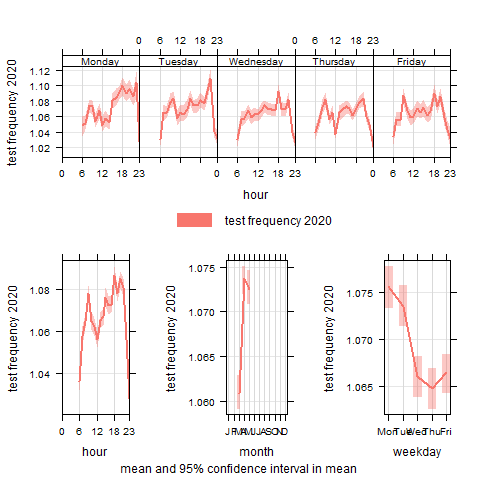
\includegraphics[width=0.75\textwidth,height=0.4\textheight]{figures/time.var.plot2020.png}
\caption{Speed tests over time, 2020 \label{test2020}}
\end{figure}

\begin{figure}
\centering
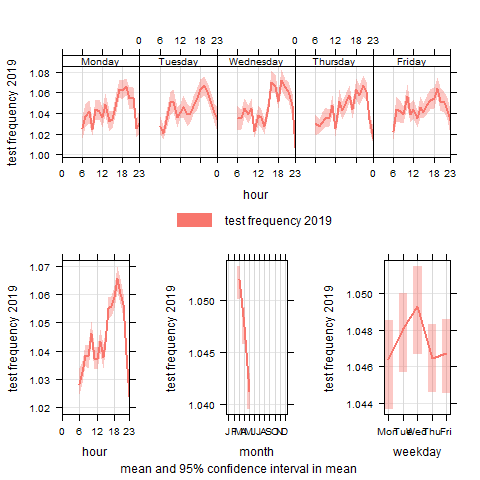
\includegraphics[width=0.75\textwidth,height=0.4\textheight]{figures/time.var.plot2019.png}
\caption{Speed tests over time, 2019 \label{test2019}}
\end{figure}

In Section \protect\hyperlink{sec:4.1}{4.1}, we review the temporal
profile of upload speed by hour of the day and day of the composite week
for each cluster. Since the quality and reliability of internet services
vary in time and space due to both supply and demand-side influences, we
also use a number of different measures to describe experienced upload
speeds per cluster. These include: i) mean, experienced connection
speed, ii) standard deviation or the amount of fluctuation from the
mean, and iii) the variation in speeds during the new morning peak of
testing when working from home is more likely to take place. We take
account of all three measurements in order to determine how resilient
broadband speeds are as experienced in different parts of the UK during
a time of extreme demand.

The cause of these different experiences of broadband resilience may
vary across different areas, as they may reflect either similarities in
patterns of demand or similar quality of infrastructure. Our approach is
also limited by potential endogeneity, as for example, better quality
connections with high mean speeds may enable more working from home, but
greater demand may cause slower speeds, less reliability and greater
variability of speed at different times of day or week. Therefore, we
avoid attributing any cause to our analysis of the experienced level of
quality and reliability of upload speeds. Instead, we run an auxiliary
regression to understand how the spatial and temporal patterns of
internet service relate to the economic geography of the UK. More
specifically, we estimate the following multinomial logit model:

\begin{align}
Pr(Y_{i}=j) = \frac{exp^{X_{i}\beta_{j}}}{\sum_{i=1}^j exp^{X_{i}\beta_{j}}}
\begin{cases}
    i = 1, 2, ... , N \\  
    j = 1, 2, ... , J
\end{cases}\label{eq1}
\end{align}

Based on the outcomes of the time-series clustering, we identify \(J\)
distinct and crisp clusters. We then regress this cluster membership
against a vector \(X_{i}\) of socio-economic and geographic variables,
which are discussed in detail in the relevant Section
\protect\hyperlink{sec:4.2}{4.2}. Because we cannot identify individuals
or households and, consequently, we aggregated our data at the LAD
level, our results offer correlations between the socioeconomic
characteristics of certain geographic locations and internet service
quality, not a record of who was telecommuting. Such individual data
could be found though surveys, but these offer less detailed information
about the experience of internet resilience due to enforced demand,
which is the main contribution of this paper. Our auxiliary regression,
therefore, provides an indication of how internet connectivity can
reinforce or redress existing spatial and social inequalities in
different places. However, it opens a path to future research by
highlighting the importance of\\
understanding of how telecommuting capabilities and digital
infrastructure divisions intersect.

\hypertarget{sec:4}{%
\section{Results}\label{sec:4}}

\hypertarget{sec:4.1}{%
\subsection{Upload Clusters / cluster description}\label{sec:4.1}}

The temporal profiles of the local authority clusters have been
summarised in Figures \ref{UpClusterL} and \ref{UpClusterS} and Table
\ref{up.cluster.descr}. The graphs show a composite profile of mean
upload speeds per hour per day for each cluster, with the largest, in
terms of the LAD membership and population, five clusters in Figure
\ref{UpClusterL}, and the next six in Figure \ref{UpClusterS}. These
figures and table provide a comprehensive overview of the quality and
reliability of experienced broadband in different parts of the UK.

\begin{figure}
\includegraphics[width=0.95\linewidth]{figures/upClusterL} \caption{\label{UpClusterL}Temporal profilies for upload speed large clusters}\label{fig:unnamed-chunk-2}
\end{figure}

\begin{figure}
\includegraphics[width=0.95\linewidth]{figures/upClusterS} \caption{\label{UpClusterS}Temporal profilies for upload speed small clusters}\label{fig:unnamed-chunk-3}
\end{figure}

\begin{table}[!htbp] \centering 
  \caption{Upload speed cluster characteristics\label{up.cluster.descr}} 
  \label{} 
\footnotesize 
\begin{tabular}{@{\extracolsep{0pt}} ccccccc} 
\\[-1.8ex]\hline 
\hline \\[-1.8ex] 
Cluster & N. of LADs & LAD population & mean speed & SD speed & mean AM speed & mean PM speed \\ 
\hline \\[-1.8ex] 
1 & 5 & 343100 & 8557 & 6139 & 7747 & 9563 \\ 
2 & 2 & 265600 & 10922 & 6687 & 9674 & 10645 \\ 
3 & 4 & 474700 & 10201 & 5658 & 9470 & 11236 \\ 
4 & 1 & 91100 & 9689 & 6122 & 7816 & 9689 \\ 
5 & 1 & 79800 & 10127 & 6024 & 9030 & 11101 \\ 
6 & 155 & 29535700 & 9397 & 5839 & 9161 & 9580 \\ 
7 & 4 & 559800 & 10119 & 6102 & 9813 & 11070 \\ 
8 & 5 & 436300 & 9429 & 6254 & 8682 & 10434 \\ 
9 & 32 & 6355500 & 10878 & 5957 & 10832 & 11071 \\ 
10 & 4 & 699600 & 10795 & 6005 & 9258 & 10697 \\ 
11 & 33 & 5771400 & 10845 & 5936 & 10781 & 10988 \\ 
12 & 10 & 1544900 & 9551 & 6166 & 9254 & 9048 \\ 
13 & 126 & 20277700 & 8392 & 5849 & 8299 & 8522 \\ 
\hline \\[-1.8ex] 
\multicolumn{7}{l}{Note: All speed measures are upload speeds} \\ 
\end{tabular} 
\end{table}

The second largest cluster, comprising \(126\) local authorities and
over \(20\) million people, is cluster \(13\), which has the slowest
aggregate mean upload speed, and the second highest ratio of the
standard deviation to the mean. This suggests that those living in local
authorities in this cluster experienced some of the lowest quality
broadband services in terms of upload speeds in the UK. However, Figure
\ref{UpClusterL} shows that the high standard deviation, which is one
indication of unreliable internet, did not disproportionately affect the
morning peak from \(9:00\)-\(10:59\), when upload speeds were, on
average, only \(2.6\)\% slower than in the evening peak period between
\(19:00\) and \(20:59\), when entertainment purposes are likely to be
using the most bandwidth. In comparison, the five LADs in cluster \(1\),
home to \(343\) thousand people, not only experience the second slowest
mean upload speeds and the highest ratio of standard deviation to the
mean, but are also much more affected during the morning peak.

Meanwhile, those living in the largest cluster -- \(6\), with \(155\)
LADs and \(29.5\) million people -- experienced aggregate mean upload
speeds of about \(1\)Mb/s faster than those in cluster \(13\), but still
lower than the other three large clusters and most of the smaller
clusters, suggesting a middling quality of service. The temporal profile
for cluster \(6\) in Figure \ref{UpClusterL} shows that upload speeds
are highest at \(6:00\) on a Monday morning and peak between \(23:00\)
and midnight on Wednesday and Thursday, but tend to be lower during the
working day. Furthermore, experienced mean upload speeds in the morning
peak are \(4.4\)\% lower than in the evening peak -- a greater, more
noticeable change than any of the other large clusters experience,
suggesting poorer reliability during the working day. This difference is
less, however than any of the clusters as shown in Figure
\ref{UpClusterS}.

Clusters \(8\) and \(12\) also have mean upload speeds under \(10\)Mb/s,
but higher than clusters \(1\), \(13\), and \(6\). However, mean upload
speeds are much lower between \(9:00-10:59\) than between
\(19:00-20:59\) in cluster \(8\), but slightly faster in the morning
than in the evening in cluster \(12\). Indeed, cluster \(12\) is the
only cluster to experience higher speeds in the morning peak compared to
the evening, and thus the only cluster where the temporal profile of
internet use is closer to what might have been expected pre-pandemic.
And yet even among the other clusters, the reliability of internet
services during the working day still varies considerably. Interpreting
this variation from the large spikes and dips shown on Figures
\ref{UpClusterL} and \ref{UpClusterS} is difficult, but the statistics
in Table \ref{up.cluster.descr} show that clusters \(9\) and \(11\) have
the most reliable internet services. The ratio of standard deviation to
mean in both these clusters is lowest, and speeds are only about 2\%
slower in the morning than the evening. Mean speeds are also higher than
in any other cluster, excluding cluster \(2\), where measures of
reliability suggests poorer performance.

Thus, broadband services in clusters \(9\) and \(11\), home to over
twelve million people performed the best during the study period, in
terms of both quality and reliability. In Figure \ref{UpClusterL},
cluster \(11\) shows more noticeable peaks and troughs, but the lowest
points are not during the morning peak, but occur, on average, between
\(6:00-7:00\) on Monday morning, \(14:00-15:00\) on Friday, and
\(16:00-17:00\) on Thursday. These slow periods still offer better
speeds than the average hourly profile of cluster \(13\). Finally,
ignoring the smallest clusters in terms of population, that is clusters
\(4\) and \(5\), clusters \(3\), \(7\) and \(10\) also have relatively
high mean upload speeds. Clusters \(3\) and \(10\) pair high mean speeds
with low standard deviations relative to the mean speeds, suggesting
reliability and resilience, as well as quality broadband services.
Cluster \(7\) has a higher ratio of standard deviation to mean, but
there is less difference in average speeds between the morning and
evening peaks than in clusters \(3\) and \(10\).

In summary, LADs in clusters \(9\) and \(11\) experienced resilient
broadband internet that could support high levels of telecommuting.
Those in clusters \(2\), \(3\), \(7\), and \(10\) also experience higher
than average mean speeds and rank middle to high on measures of service
reliability. These LADs are \emph{not} on the wrong side of the first
level digital divide, but how likely are they to be able to take
advantage of their resilient ICT infrastructure and services? Meanwhile,
cluster \(6\) is not only the largest in terms of number of LADs and
population, it has the closest mean upload speed to the pre-clustered
average for the whole sample. As well as average quality internet
services, those in cluster \(6\) also experience average reliability for
work purposes, ranking fifth behind the four other clusters with
populations over one million, but ahead of the smaller clusters.
Clusters \(8\) and \(12\) are also close to average mean upload speeds,
but show very different patterns in terms of reliability, whilst
clusters \(1\) and \(13\) appear to suffer most from a lack of quality
internet services, with slow speeds and high standard deviations. With
those in cluster \(1\) more likely to experience that poor reliability
during the morning peak, is this first level digital divide occurring in
areas where few are occupationally able to telecommute anyway, and what
are the implications for economic resilience?

\hypertarget{sec:4.2}{%
\subsection{Post-clustering regression analysis}\label{sec:4.2}}

\begin{sidewaystable}[!htbp] \centering 
  \caption{Auxiliary multinomial regression of upload speed clusters on socio-economic and geographic LAD variables\label{aux}} 
  \label{} 
\tiny 
\begin{tabular}{@{\extracolsep{5pt}}lccccccccccc} 
\\[-1.8ex]\hline 
\hline \\[-1.8ex] 
\\[-1.8ex] & 1 & 2 & 3 & 6 & 7 & 8 & 9 & 10 & 11 & 12 & 13 \\ 
\\[-1.8ex] & (1) & (2) & (3) & (4) & (5) & (6) & (7) & (8) & (9) & (10) & (11)\\ 
\hline \\[-1.8ex] 
 pop, 2018 & $-$0.00004$^{***}$ & 0.00002$^{*}$ & 0.00001 & 0.00002$^{***}$ & 0.00002$^{***}$ & 0.00000 & 0.00002$^{***}$ & 0.00002$^{***}$ & 0.00002$^{***}$ & 0.00002$^{**}$ & 0.00002$^{***}$ \\ 
  & (0.00002) & (0.00001) & (0.00001) & (0.00001) & (0.00001) & (0.00002) & (0.00001) & (0.00001) & (0.00001) & (0.00001) & (0.00001) \\ 
  & & & & & & & & & & & \\ 
 job density, 2018 & $-$0.536$^{***}$ & $-$1.834$^{***}$ & $-$0.132$^{***}$ & $-$0.925$^{***}$ & $-$1.208$^{***}$ & $-$0.299$^{***}$ & $-$1.746$^{***}$ & $-$1.436$^{***}$ & 3.350$^{***}$ & 3.400$^{***}$ & 0.630$^{***}$ \\ 
  & (0.00000) & (0.00000) & (0.00000) & (0.00000) & (0.00000) & (0.00000) & (0.00000) & (0.00000) & (0.00000) & (0.00000) & (0.00000) \\ 
  & & & & & & & & & & & \\ 
 distance to nearest met. area & $-$0.034$^{***}$ & $-$0.014$^{***}$ & 0.002$^{***}$ & $-$0.020$^{***}$ & $-$0.074$^{***}$ & $-$0.044$^{***}$ & $-$0.013$^{***}$ & $-$0.036$^{***}$ & $-$0.031$^{***}$ & $-$0.036$^{***}$ & $-$0.024$^{***}$ \\ 
  & (0.0005) & (0.001) & (0.0002) & (0.002) & (0.0001) & (0.0002) & (0.002) & (0.0005) & (0.0003) & (0.0002) & (0.002) \\ 
  & & & & & & & & & & & \\ 
 distance to London & 0.007$^{***}$ & 0.002 & $-$0.016$^{***}$ & 0.001 & 0.004$^{***}$ & 0.004$^{***}$ & $-$0.002$^{*}$ & 0.005$^{**}$ & $-$0.002 & 0.003 & 0.006$^{***}$ \\ 
  & (0.001) & (0.002) & (0.0004) & (0.001) & (0.001) & (0.001) & (0.001) & (0.002) & (0.002) & (0.002) & (0.001) \\ 
  & & & & & & & & & & & \\ 
 South of the UK & $-$0.410$^{***}$ & $-$1.451$^{***}$ & $-$0.039$^{***}$ & $-$0.111$^{***}$ & $-$0.048$^{***}$ & $-$0.841$^{***}$ & $-$0.798$^{***}$ & 1.492$^{***}$ & 0.610$^{***}$ & 0.798$^{***}$ & 2.403$^{***}$ \\ 
  & (0.00000) & (0.00000) & (0.00000) & (0.00001) & (0.00000) & (0.00000) & (0.00001) & (0.00000) & (0.00001) & (0.00001) & (0.00001) \\ 
  & & & & & & & & & & & \\ 
 managerial jobs, 2020 & 0.939$^{***}$ & 0.704$^{***}$ & 0.435$^{***}$ & 0.704$^{***}$ & 0.316$^{***}$ & 0.786$^{***}$ & 0.576$^{***}$ & 0.311$^{***}$ & 0.476$^{***}$ & 0.594$^{***}$ & 0.615$^{***}$ \\ 
  & (0.00004) & (0.0001) & (0.00004) & (0.00004) & (0.00002) & (0.0001) & (0.00003) & (0.00003) & (0.00002) & (0.00004) & (0.00003) \\ 
  & & & & & & & & & & & \\ 
 tech jobs, 2020 & 0.096$^{***}$ & $-$0.257$^{***}$ & $-$0.071$^{***}$ & $-$0.111$^{***}$ & $-$0.206$^{***}$ & 0.199$^{***}$ & $-$0.126$^{***}$ & $-$0.606$^{***}$ & $-$0.180$^{***}$ & $-$0.398$^{***}$ & $-$0.112$^{***}$ \\ 
  & (0.00004) & (0.00004) & (0.00004) & (0.00003) & (0.00003) & (0.0001) & (0.00003) & (0.00003) & (0.00002) & (0.00004) & (0.00003) \\ 
  & & & & & & & & & & & \\ 
 skilled trade jobs, 2020 & 0.651$^{***}$ & 0.160$^{***}$ & $-$0.191$^{***}$ & 0.236$^{***}$ & 0.604$^{***}$ & $-$0.184$^{***}$ & 0.205$^{***}$ & 0.597$^{***}$ & 0.108$^{***}$ & $-$0.022$^{***}$ & 0.295$^{***}$ \\ 
  & (0.00004) & (0.00004) & (0.00003) & (0.00003) & (0.00003) & (0.00004) & (0.00002) & (0.00003) & (0.00003) & (0.00004) & (0.00003) \\ 
  & & & & & & & & & & & \\ 
 professional jobs, 2020 & $-$0.118$^{***}$ & $-$0.234$^{***}$ & $-$0.121$^{***}$ & $-$0.172$^{***}$ & $-$0.514$^{***}$ & $-$0.172$^{***}$ & $-$0.349$^{***}$ & $-$0.351$^{***}$ & $-$0.245$^{***}$ & $-$0.344$^{***}$ & $-$0.229$^{***}$ \\ 
  & (0.00005) & (0.0001) & (0.0001) & (0.00005) & (0.00003) & (0.0001) & (0.00004) & (0.0001) & (0.00003) & (0.00005) & (0.0001) \\ 
  & & & & & & & & & & & \\ 
 administrative jobs, 2020 & 0.019$^{***}$ & $-$0.836$^{***}$ & $-$0.040$^{***}$ & $-$0.117$^{***}$ & $-$0.139$^{***}$ & 0.206$^{***}$ & $-$0.058$^{***}$ & $-$0.200$^{***}$ & $-$0.055$^{***}$ & $-$0.168$^{***}$ & $-$0.177$^{***}$ \\ 
  & (0.00003) & (0.00002) & (0.00004) & (0.00001) & (0.00003) & (0.00003) & (0.00001) & (0.00002) & (0.00002) & (0.00002) & (0.00002) \\ 
  & & & & & & & & & & & \\ 
 leisure jobs, 2020 & $-$0.198$^{***}$ & $-$0.180$^{***}$ & $-$0.225$^{***}$ & $-$0.476$^{***}$ & $-$0.654$^{***}$ & $-$0.820$^{***}$ & $-$0.537$^{***}$ & $-$0.935$^{***}$ & $-$0.353$^{***}$ & $-$0.625$^{***}$ & $-$0.491$^{***}$ \\ 
  & (0.00002) & (0.00004) & (0.00004) & (0.00002) & (0.00002) & (0.00003) & (0.00002) & (0.00001) & (0.00002) & (0.00003) & (0.00002) \\ 
  & & & & & & & & & & & \\ 
 machine operation jobs, 2020 & $-$0.336$^{***}$ & 0.207$^{***}$ & 0.392$^{***}$ & 0.010$^{***}$ & $-$0.433$^{***}$ & 0.139$^{***}$ & $-$0.099$^{***}$ & $-$0.139$^{***}$ & $-$0.144$^{***}$ & 0.098$^{***}$ & $-$0.179$^{***}$ \\ 
  & (0.00002) & (0.00003) & (0.00003) & (0.00002) & (0.00001) & (0.00003) & (0.00002) & (0.00001) & (0.00001) & (0.00002) & (0.00001) \\ 
  & & & & & & & & & & & \\ 
 earnings, 2019 & $-$0.003$^{*}$ & 0.010$^{***}$ & 0.012$^{***}$ & 0.020$^{***}$ & 0.027$^{***}$ & 0.001 & 0.020$^{***}$ & 0.016$^{***}$ & 0.015$^{***}$ & 0.025$^{***}$ & 0.014$^{***}$ \\ 
  & (0.002) & (0.002) & (0.002) & (0.001) & (0.001) & (0.003) & (0.001) & (0.002) & (0.001) & (0.001) & (0.001) \\ 
  & & & & & & & & & & & \\ 
 n. business est. per hab., 2019 & 0.126$^{***}$ & $-$0.120$^{***}$ & $-$0.094$^{***}$ & $-$0.133$^{***}$ & 0.123$^{***}$ & $-$0.051$^{***}$ & $-$0.334$^{***}$ & $-$0.133$^{***}$ & $-$0.150$^{***}$ & 0.289$^{***}$ & 0.377$^{***}$ \\ 
  & (0.00000) & (0.00000) & (0.00000) & (0.00000) & (0.00000) & (0.00000) & (0.00000) & (0.00000) & (0.00000) & (0.00000) & (0.00000) \\ 
  & & & & & & & & & & & \\ 
 NVQ4+ & $-$0.141$^{***}$ & 0.064$^{***}$ & $-$0.091$^{***}$ & $-$0.070$^{***}$ & $-$0.010$^{***}$ & 0.004$^{***}$ & 0.016$^{***}$ & 0.170$^{***}$ & $-$0.110$^{***}$ & $-$0.038$^{***}$ & $-$0.035$^{***}$ \\ 
  & (0.0001) & (0.0001) & (0.0001) & (0.0001) & (0.0001) & (0.0002) & (0.0001) & (0.0001) & (0.0001) & (0.0001) & (0.0001) \\ 
  & & & & & & & & & & & \\ 
 AM tests per hab., 2020 & 0.0005$^{***}$ & $-$0.002$^{***}$ & $-$0.005$^{***}$ & 0.010$^{***}$ & 0.0004$^{***}$ & $-$0.001$^{***}$ & $-$0.002$^{***}$ & $-$0.005$^{***}$ & $-$0.013$^{***}$ & $-$0.001$^{***}$ & 0.016$^{***}$ \\ 
  & (0.000) & (0.000) & (0.000) & (0.000) & (0.000) & (0.000) & (0.000) & (0.000) & (0.000) & (0.000) & (0.000) \\ 
  & & & & & & & & & & & \\ 
 Virgin Media \%, 2020 & $-$0.044$^{***}$ & 1.578$^{***}$ & 1.210$^{***}$ & 0.248$^{***}$ & $-$1.724$^{***}$ & $-$0.242$^{***}$ & 3.109$^{***}$ & $-$0.085$^{***}$ & 1.214$^{***}$ & $-$3.889$^{***}$ & $-$0.745$^{***}$ \\ 
  & (0.00000) & (0.00000) & (0.00000) & (0.00000) & (0.00000) & (0.00000) & (0.00000) & (0.00000) & (0.00000) & (0.00000) & (0.00000) \\ 
  & & & & & & & & & & & \\ 
 Constant & 0.321$^{***}$ & $-$0.436$^{***}$ & 0.199$^{***}$ & $-$2.953$^{***}$ & 0.278$^{***}$ & 0.002$^{***}$ & $-$0.866$^{***}$ & 0.788$^{***}$ & 2.600$^{***}$ & 0.017$^{***}$ & 0.022$^{***}$ \\ 
  & (0.00000) & (0.00000) & (0.00000) & (0.00000) & (0.00000) & (0.00000) & (0.00000) & (0.00000) & (0.00000) & (0.00000) & (0.00000) \\ 
  & & & & & & & & & & & \\ 
\hline \\[-1.8ex] 
McFadden's R squared & 0.338 & 0.338 & 0.338 & 0.338 & 0.338 & 0.338 & 0.338 & 0.338 & 0.338 & 0.338 & 0.338 \\ 
N & 323 & 323 & 323 & 323 & 323 & 323 & 323 & 323 & 323 & 323 & 323 \\ 
Akaike Inf. Crit. & 1,148.027 & 1,148.027 & 1,148.027 & 1,148.027 & 1,148.027 & 1,148.027 & 1,148.027 & 1,148.027 & 1,148.027 & 1,148.027 & 1,148.027 \\ 
\hline 
\hline \\[-1.8ex] 
\textit{Note:}  & \multicolumn{11}{r}{$^{*}$p$<$0.1; $^{**}$p$<$0.05; $^{***}$p$<$0.01} \\ 
\end{tabular} 
\end{sidewaystable}

Using an auxiliary multinomial regression, we test whether the clusters
that have higher mean speeds and more reliable services consist of LADs
that are more urban, affluent, and / or more likely to benefit from a
choice of high quality internet services. We also estimate which of our
clusters are more likely to have a higher proportion of occupations
which enable telecommuting because of the nature of the work. The
results of the auxiliary regression are presented in Table \ref{aux}.
The dependent variable is the LAD cluster membership as described in the
\protect\hyperlink{sec:3}{methods and data} section and equation
\ref{eq1} and each column represent a different cluster. The reference
case is cluster \(4\), which includes only the local authority of
Hambleton in North Yorkshire, a rural area of just over ninety thousand
people. Mean, experienced upload speeds in cluster \(4\) (see Table
\ref{up.cluster.descr}) are close to both the average speeds for the
\(13\) clusters (\(9.9\)Mb/s) and the pre-clustered average for the
whole sample (\(9.3\)Mb/s). However, the standard deviation for cluster
\(4\) and the difference between average speeds in the morning compared
to the evening peak periods are indications of worse reliability than
many of the other clusters. Hence, the results in Table \ref{aux} should
be seen as relative rather than absolute probabilities.

First, we control for the number of speed tests run per cluster
inhabitant between \(9:00\)-\(10:59\) as well as the share of fast
Virgin Media internet connections. Regarding the former, we expect
people in LADs with more unreliable connections to test their internet
speeds more often, and the results validate our priors. Meanwhile, fast
Virgin Media cable connections have historically only been available to
\(45\)\% of premises in the UK \citep{ofcom2016}, where the more
lucrative and competitive market originally attracted the cable TV
provider. Those in clusters \(2\), \(3\), \(9\) and \(11\) benefit from
a higher proportion of Virgin connections, which is an indication that
people in these clusters are more likely to live in urban areas, with
more choice of broadband services, or in other words, are more likely to
be on the right side of the first level, infrastructure-based digital
divide, as we expected from the analysis in Section
\protect\hyperlink{sec:4.1}{4.1}.

Then, we employ distance from London and from the nearest metropolitan
area (including London) as two variables depicting peripherality, urban
structure and, potentially, first level digital divides. The broadband
speed tests run in the authorities in cluster \(3\) are more likely to
be taking place close to London than those run in any of the other
clusters, and two of the four authorities in cluster \(3\) are the
London commuter towns of Harlow and Luton. However, even though London
was also included in the variable calculating distance from the centre
of one of either the ten largest metropolitan areas in England, or
Glasgow or Cardiff, tests run in cluster \(3\) are likely to be furthest
away. Thus, it is important to consider the membership of each cluster
as well as the regression results. Corby and Eastbourne, the other two
authorities in cluster \(3\) are, whilst not part of metropolitan areas,
are also large, accessible towns.

\begin{figure}
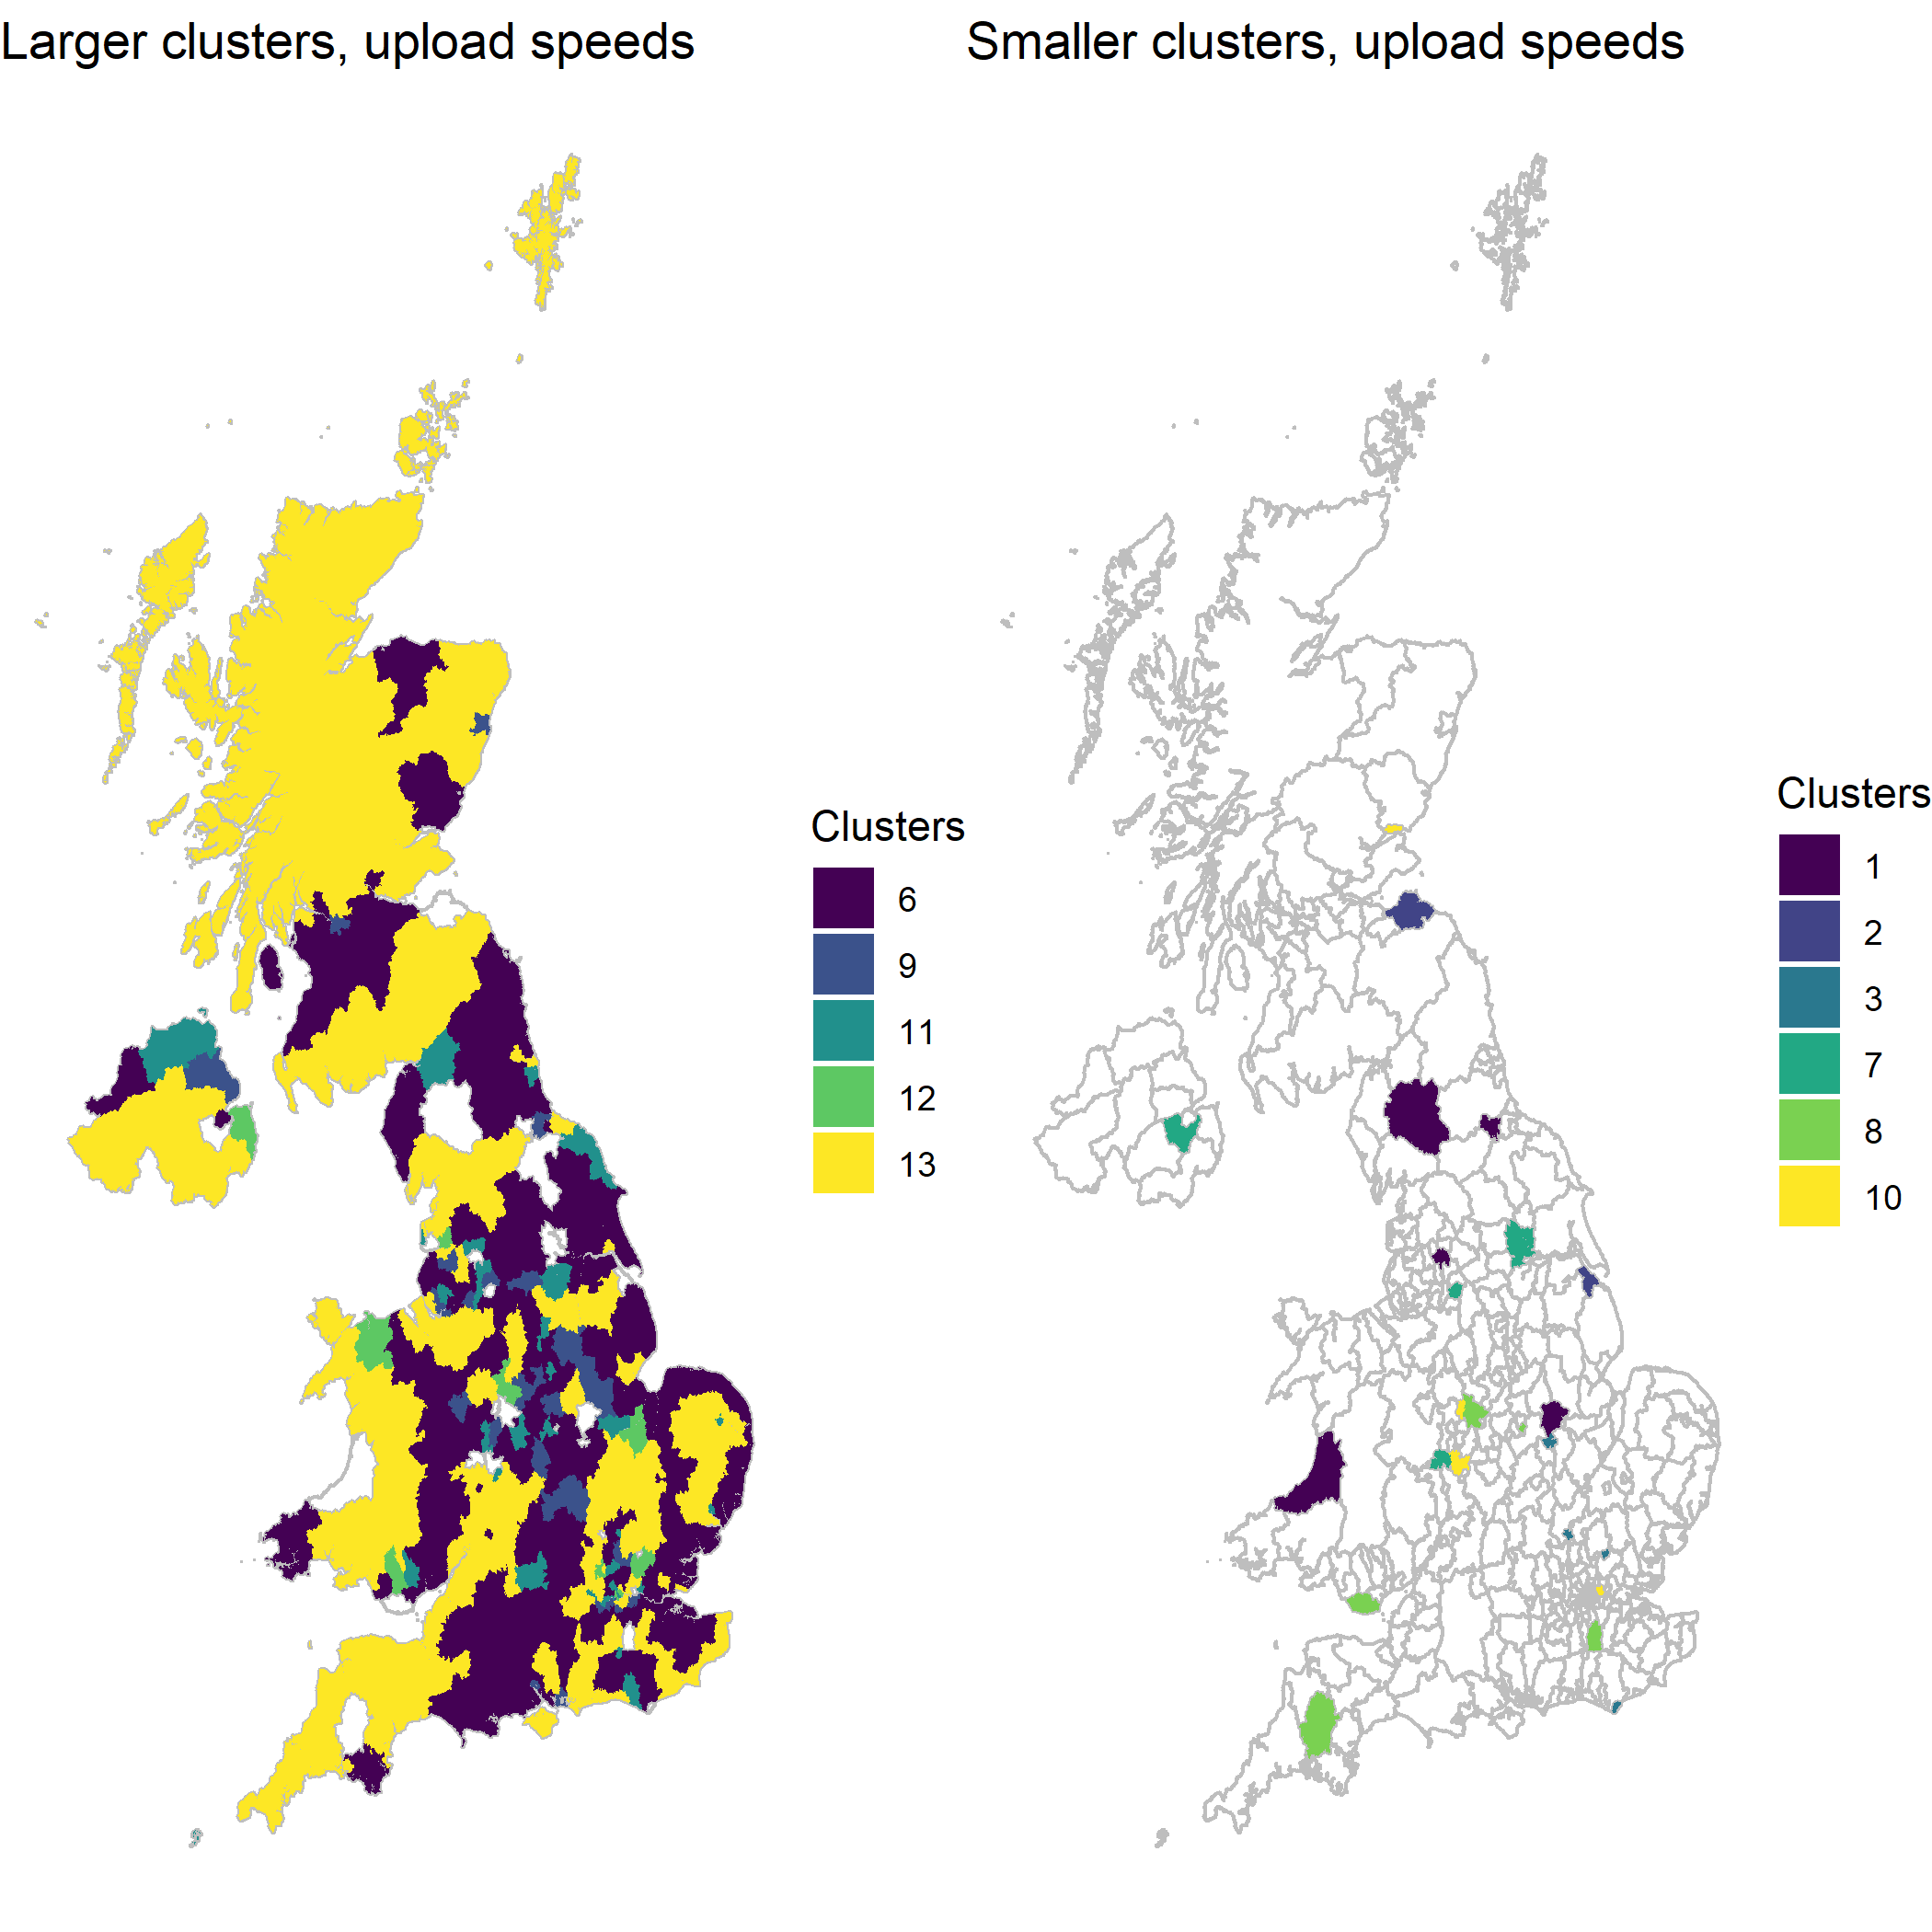
\includegraphics[width=0.95\linewidth]{figures/map.up.clusters} \caption{\label{map.up.clusters}Upload speed clusters for LADs}\label{fig:unnamed-chunk-6}
\end{figure}

Meanwhile, LADs in cluster \(7\) are most likely to be near the centre
of a large metropolitan area, even though the four local authorities of
cluster \(7\) include no central urban boroughs and only one LAD that is
part of a metropolitan area of governance - Tameside in Greater
Manchester. This may explain why those in cluster \(7\) are the second
least likely to be served by Virgin Media. It is also a demonstration of
the complexity of experienced broadband upload speeds as captured by
time-series clustering, and how quality and reliability, not only
availability, engender first level digital divides. Cluster \(1\), which
our analysis suggests lacks broadband resilience, contains five, mainly
rural authorities. However, they are scattered around the country --
Ceredigion in West Wales, Darlington in the Northeast, Eden and
Rossendale in the Northwest, and Rutland in the East Midlands -- and
therefore, the results in Table \ref{aux} indicate that these
authorities are closer to a metropolitan area than authorities in
cluster \(3\), but furthest from London.

Internet resilience is also more nuanced than our -- arguably crude --
dummy variable depicting the North-South economic divide, which assigns
\(1\) to LADs located in Greater London, Southeast, Southwest and East
of England regions, and \(0\) to the rest. The authorities most likely
to be in the South are those in cluster \(13\), which was identified as
having the slowest mean upload speeds of any of the clusters, and thus a
low level of service. However, cluster \(13\) includes some rural,
remote areas of the country, such as Northwest Scotland, Cornwall and
Powys in Wales as shown on Figure \ref{map.up.clusters}. It also
includes major metropolitan centres in the North -- Liverpool, Newcastle
-- and South -- Bristol, nine (of \(32\)) London Boroughs. There are
also plenty of Southern home county and suburban areas. The standard
deviation measure for cluster \(13\) is high, but speed variation is low
during the morning peak, suggesting that the estimates for reliability
are inconsistent. Considering that this is one of the largest clusters,
and thus the averages incorporate more noise than some of the smaller
clusters, it may be that the LADs in this cluster do not all suffer
equally from a first level digital divide.

Yet we need to consider the results for other variables in Table
\ref{aux} to better determine whether clusters \(1\) and \(13\), which
appear to suffer most from poor quality internet services, are also more
likely to have a low skilled workforce, less able to benefit from
telecommuting. Cluster \(1\) has the lowest proportion of educated
people, and the lowest earnings, despite recording the highest
proportion of managerial, professional jobs, and the second highest
proportion of tech jobs. Rural areas such as those in cluster \(1\) are
often home to many retired people, which might explain these results or
perhaps, as these figures are relative, we could note that cluster \(1\)
also has a greater proportion of skilled trades than other clusters. It
seems likely that the first level digital divide reinforces other
inequities in cluster \(1\), whilst those in cluster \(13\) are more
likely to earn more and have a better education despite poor internet
services. Cluster \(13\) also has the most businesses per inhabitant,
but is somewhere in the middle in terms of job density. If this is an
indication of a high number of SMEs, it could explain the variable
internet quality, considering that small businesses have not been seen
as the most valuable customers for higher speed broadband services if
they are not located near residential customers \citep{ofcom2016}.

Cluster \(6\) is the largest cluster, and thus, like cluster \(13\),
there is more noise within the averages we use to measure internet
quality and reliability. Our results indicate average mean speeds, and
Table \ref{aux} shows that cluster \(6\) also falls towards the middle
of the clusters on many of the socioeconomic variables. It ranks third
or fourth out of the eleven in terms of the likelihood of having a
higher proportion of managerial, professional, and tech jobs, as well as
higher earnings, but is fourth from bottom for educational attainment.
The LADs in cluster \(6\) are also diverse, with few truly remote areas,
but urban areas throughout England, including Birmingham, Leeds,
Sheffield, twelve London Boroughs, and many suburban areas and smaller
cities like Oxford and Cambridge. The capital cities of the other UK
nations, Belfast, Cardiff and Edinburgh, are also in this cluster,
suggesting perhaps that the lower level of reliability discussed in
Section \protect\hyperlink{sec:4.1}{4.1} may be due to increased demand,
e.g.~for telecommuting, when it is not supported by the most resilient
internet connections.

In contrast, Clusters \(9\) and \(11\) enjoy resilient internet
connections and are characterised by higher share of occupations that
may benefit from the ability to telecommute (e.g.~managerial). LADs in
Cluster \(9\) are more likely to host highly educated individuals with
higher earnings than cluster \(11\), which has a negative coefficient
for the NVQ4 variable. Cluster \(11\) has fewer businesses per
inhabitant and the second highest job density and cluster \(9\) the
second lowest. These coefficients might indicate that resilient
broadband infrastructure generates higher returns for those in cluster
\(9\), where slightly more slowdown in the AM peak was detected (see
Table \ref{up.cluster.descr}). LADs in cluster \(9\) are also less
likely to be in the South and those in cluster \(11\) more likely,
although the coefficient for cluster \(9\) might be skewed by the
presence of the Scottish cities of Glasgow and Aberdeen. Scotland has a
different economic profile than England. Still, both clusters consist of
larger LADs in terms of population, including the city centre among four
of the ten districts of Greater Manchester, eight London Boroughs, four
of the seven constituent authorities of the West Midlands Combined
Authority, Nottingham, and both Portsmouth and Southampton. Among the
\(65\) LADs are also a number of other tightly bounded urban areas, such
as Blackpool, Ipswich, Norwich, Slough, and Stevenage, and urban areas
at the centre of less confined districts like Burnley, the digital hub
of Milton Keynes, and Northampton. These urban locations are on the
right side of the first level digital divide, and the regression results
suggest that internet resilience is supporting a wide range of small and
large urban economies.

LADs in clusters \(2\), \(3\), \(7\), \(10\) are also on the right side
of the first level digital divide, experiencing higher than average mean
speeds and ranking high to middle on measures of service reliability.
However, only LADs in cluster \(2\) and \(10\) are more likely to have
highly skilled work force to take advantage of working from home
opportunities. Cluster \(2\) is comprised of just two LADs, with the
lowest job density of any cluster -- these are East Lothian near
Edinburgh, and North East Lincolnshire, home to the town of Grimsby.
Cluster \(10\) is comprised of four LADs, including two peripheral
suburban areas of Birmingham, the East London Borough of Newham, and
Dundee. Suburbs are considered the most likely urban form in which
telecommuters live \citep{e2018does}, and Dundee has a reputation for
tech startups \citep{technation2017}. LADs in cluster \(7\), which
include the suburbs South of Belfast, a suburban district of Greater
Manchester, the villages between York and Leeds, and a couple of small
West Midlands towns have the highest earnings, and thus may also be
making the most of their resilient internet. In contrast, LADs in
cluster \(3\) are associated more with lower skills and have the highest
proportion of individuals in machine operation jobs. Arguably, LADs in
clusters \(3\) benefit the least from their resilient internet
infrastructure in an era when working from home became a vehicle for
economic resilience.

Finally, clusters \(8\) and \(12\) consist by LADs enjoying close to
average mean upload speeds, but opposing patterns of internet
reliability during the morning peak. LADs in cluster \(8\) are likely to
host more individuals employed in tech and administrative occupations
than any other cluster, as well as many in managerial occupations,
whilst the opposite applies to skilled trade and leisure occupations.
These LADs are characterised by a very small positive likelihood of more
educated residents, but are not significantly likely to earn more than
other clusters. Including suburbs near Leicester, Cardiff, Birmingham,
the green belt area south of London straddling the M25 motorway, and
rural West Devon, the LADs in cluster \(8\) seem to likely to have the
skills and occupations that would benefit from quality internet
services, but suffer from poor internet resilience and reliability.

In comparison, LADs in cluster \(12\) are less likely to be able to
benefit from quality internet services if they had them, with fewer
individuals achieving NVQ4 or better and lower levels of occupations
that would benefit from homeworking. Yet LADs in this cluster benefit
from the second highest level of earnings, and have the largest stock of
businesses per inhabitant and the highest job density. This density of
businesses could be why cluster \(12\) is the only cluster with higher
speeds in the morning peak during the study period. If people are at
home, business premises might well have been abandoned. Cluster \(12\)
is home to \(1.5\) million people spread across twelve LADs, including
the City of Westminster but also a LAD in Northern Ireland, two in
Wales, Preston in the Northwest, and Fenland in the East of England.
This spatial diversity demonstrates that the temporal clustering of
internet resilience is not necessarily spatially dependent, and digital
divides do not necessarily overlap with economic ones.

\hypertarget{sec:5}{%
\section{Conclusions}\label{sec:5}}

This paper offers a new perspective on telecommuting from the viewpoint
of the complex web of digital divides. To do so, we employ novel data
regarding experienced upload speeds and time-series clustering methods,
a family of unsupervised machine learning techniques which are rarely
utilised in geographical research. Fast, reliable internet connections
are necessary for the population to be able to work from home. Although
not every place hosts individuals in occupations which allow for
telecommuting nor with the necessary skills to effectively use the
internet to telecommute, this paper raises the issue that without good
internet connectivity, these places would struggle more to achieve
economic resilience in a period like the current pandemic in any case.
Indeed, our analysis demonstrated that the temporal profiles of twelve
of our thirteen clusters had slower upload speeds in the morning than in
the evening. The opposite is likely to have been the norm prior to the
pandemic, as the level of demand and bandwidth management is the most
common cause of temporal variation in experienced speeds, and why
evening download speeds, rather than daytime upload speeds have been
used to benchmark the performance of internet services. Thus, the new
patterns can be taken as evidence of widespread telecommuting and other
daytime internet use which changed the temporal profile of internet
activity throughout the UK, not just in areas with more digital industry
or better skills.

Upload speeds have not previously been seen as integral to universal
service, considering there has never before been such extreme demand for
telecommuting and operations such as video calls. This may be why the
average upload speeds for the largest two clusters -- \(6\) and \(13\)
-- contain so many LADs that are centres of the knowledge economy, from
Oxford and Cambridge in the former, to areas like Reading, which has the
highest concentration of digital businesses in the country
\citep{technation2017}. Thus, whilst some areas suffer from an
intersection of digital and economic divides, such as those in cluster
\(1\), others found their digital infrastructure to be less reliable
when confronted with the sudden change in the timing and type of demand.
Still other LADs, such as Milton Keynes in cluster \(9\) were able to
benefit both from reliable internet connections and populations which
were familiar with working from home and could capitalise on their
digital infrastructure. Yet the nuanced picture we gained through our
analysis of the UK case study suggests that quality internet
connectivity would also enable other LADs to gain ground during the
pandemic despite lower skills or earnings currently, especially in a
future where telecommuting might be a more common means of accessing
work and broadband services must be fit for purpose.

Indeed, the long-term effects of such drastic changes in telecommuting
and attitudes towards working from home are difficult to predict.
Nevertheless, they span through various aspects of economy and society:
from changes to transportation planning due to altered commuting
patterns to changes in land use and urban planning to accommodate people
who work from home \citep{BUDNITZ2020102713, ELLDER2020102777}, and from
productivity and innovation changes to changes in agglomeration
externalities and the attraction of large cities \citep{econobs}.
Further research may be able to measure the economic resilience of the
different clusters of places discussed in this paper once this pandemic
is firmly past. However, our analysis demonstrates that the economic
resilience made possible by working from home cannot be understood
without considering the underpinning digital divides and cannot be
achieved without planning for how the levels of digital, social and
economic divides might intersect.

\hypertarget{appendix1}{%
\section{Appendix 1}\label{appendix1}}

This is the LAD cluster membership for the upload speed timeseries.

\textbf{Cluster 1: } Ceredigion, Darlington, Eden, Rossendale, Rutland

\textbf{Cluster 2: } East Lothian, North East Lincolnshire

\textbf{Cluster 3: } Corby, Eastbourne, Harlow, Luton

\textbf{Cluster 4: } Hambleton

\textbf{Cluster 5: } Fylde

\textbf{Cluster 6: } Allerdale, Amber Valley, Angus, Ashfield, Ashford,
Aylesbury Vale, Barnet, Basingstoke and Deane, Bath and North East
Somerset, Belfast, Bexley, Birmingham, Blaenau Gwent, Bournemouth,
Christchurch and Poole, Bradford, Braintree, Brentwood, Bridgend,
Bromley, Broxtowe, Bury, Calderdale, Cambridge, Canterbury, Cardiff,
Castle Point, Chelmsford, Cheltenham, Cherwell, Chesterfield, City of
Edinburgh, Clackmannanshire, Colchester, Copeland, County Durham,
Coventry, Croydon, Dartford, Daventry, Denbighshire, Derby, Derry City
and Strabane, Dorset, Ealing, East Ayrshire, East Hampshire, East
Lindsey, East Northamptonshire, East Renfrewshire, East Riding of
Yorkshire, East Suffolk, Eastleigh, Elmbridge, Enfield, Falkirk,
Fareham, Gateshead, Gedling, Gosport, Gravesham, Great Yarmouth,
Guildford, Harborough, Haringey, Harrogate, Harrow, Hart, Hartlepool,
Havering, Herefordshire, County of, High Peak, Hinckley and Bosworth,
Horsham, Islington, Kettering, King's Lynn and West Norfolk, Kingston
upon Thames, Kirklees, Leeds, Leicester, Lincoln, Maidstone, Maldon,
Mansfield, Medway, Mendip, Mid Sussex, Middlesbrough, Monmouthshire,
Moray, New Forest, Newcastle-under-Lyme, Newport, North Ayrshire, North
East Derbyshire, North Hertfordshire, North Kesteven, North Lanarkshire,
North Lincolnshire, North Norfolk, North Tyneside, North West
Leicestershire, Northumberland, Nuneaton and Bedworth, Oxford,
Pembrokeshire, Pendle, Renfrewshire, Ribble Valley, Rochford, Runnymede,
Rushcliffe, Ryedale, Salford, Sefton, Sheffield, Shropshire, Solihull,
South Ayrshire, South Hams, South Holland, South Lanarkshire, South
Oxfordshire, South Staffordshire, St Albans, Staffordshire Moorlands,
Stockport, Stoke-on-Trent, Surrey Heath, Sutton, Swale, Tamworth,
Tendring, Test Valley, Thurrock, Tonbridge and Malling, Torfaen,
Wakefield, Warrington, Warwick, Wealden, Wellingborough, West Berkshire,
West Dunbartonshire, West Lancashire, West Lothian, West Oxfordshire,
West Suffolk, Wigan, Wiltshire, Woking, Worcester, Wrexham, Wycombe,
York

\textbf{Cluster 7: } Lisburn and Castlereagh, Selby, Tameside, Wyre
Forest

\textbf{Cluster 8: } Lichfield, Oadby and Wigston, Tandridge, Vale of
Glamorgan, West Devon

\textbf{Cluster 9: } Aberdeen City, Barnsley, Broxbourne, Charnwood,
Chorley, Erewash, Glasgow City, Greenwich, Halton, Havant, Knowsley,
Lewisham, Merton, Mid and East Antrim, Milton Keynes, Newark and
Sherwood, Northampton, Oldham, Portsmouth, Richmond upon Thames, Rugby,
Sandwell, South Derbyshire, South Kesteven, South Northamptonshire,
Southampton, Spelthorne, Stockton-on-Tees, Telford and Wrekin, Trafford,
Walsall, Welwyn Hatfield

\textbf{Cluster 10: } Bromsgrove, Cannock Chase, Dundee City, Newham

\textbf{Cluster 11: } Barking and Dagenham, Blaby, Blackpool, Bolsover,
Brent, Burnley, Caerphilly, Carlisle, Causeway Coast and Glens, Crawley,
Doncaster, Dudley, Hertsmere, Hounslow, Hyndburn, Ipswich, Isles of
Scilly, Kensington and Chelsea, Lewes, Manchester, North Warwickshire,
Norwich, Nottingham, Peterborough, Redditch, Rochdale, Scarborough,
Slough, St.~Helens, Stevenage, Sunderland, Vale of White Horse,
Wolverhampton

\textbf{Cluster 12: } Ards and North Down, Conwy, East Staffordshire,
Epping Forest, Fenland, Hammersmith and Fulham, Preston, Rhondda Cynon
Taf, Three Rivers, Westminster

\textbf{Cluster 13: } Aberdeenshire, Adur, Antrim and Newtownabbey,
Argyll and Bute, Armagh City, Banbridge and Craigavon, Arun, Babergh,
Barrow-in-Furness, Basildon, Bassetlaw, Bedford, Blackburn with Darwen,
Bolton, Boston, Bracknell Forest, Breckland, Brighton and Hove, Bristol,
City of, Broadland, Camden, Carmarthenshire, Central Bedfordshire,
Cheshire East, Cheshire West and Chester, Chichester, Chiltern, City of
London, Cornwall, Cotswold, Craven, Dacorum, Derbyshire Dales, Dover,
Dumfries and Galloway, East Cambridgeshire, East Devon, East
Dunbartonshire, East Hertfordshire, Epsom and Ewell, Exeter, Fermanagh
and Omagh, Fife, Flintshire, Folkestone and Hythe, Forest of Dean,
Gloucester, Gwynedd, Hackney, Hastings, Highland, Hillingdon,
Huntingdonshire, Inverclyde, Isle of Anglesey, Isle of Wight, Kingston
upon Hull, City of, Lambeth, Lancaster, Liverpool, Malvern Hills,
Melton, Merthyr Tydfil, Mid Devon, Mid Suffolk, Mid Ulster, Midlothian,
Mole Valley, Na h-Eileanan Siar, Neath Port Talbot, Newcastle upon Tyne,
Newry, Mourne and Down, North Devon, North Somerset, Orkney Islands,
Perth and Kinross, Plymouth, Powys, Reading, Redbridge, Redcar and
Cleveland, Reigate and Banstead, Richmondshire, Rother, Rotherham,
Rushmoor, Scottish Borders, Sedgemoor, Sevenoaks, Shetland Islands,
Somerset West and Taunton, South Bucks, South Cambridgeshire, South
Gloucestershire, South Lakeland, South Norfolk, South Ribble, South
Somerset, South Tyneside, Southend-on-Sea, Southwark, Stafford,
Stirling, Stratford-on-Avon, Stroud, Swansea, Swindon, Teignbridge,
Tewkesbury, Thanet, Torbay, Torridge, Tower Hamlets, Tunbridge Wells,
Uttlesford, Waltham Forest, Wandsworth, Watford, Waverley, West Lindsey,
Winchester, Windsor and Maidenhead, Wirral, Wokingham, Worthing,
Wychavon, Wyre

\hypertarget{appendix2}{%
\section{Appendix 2}\label{appendix2}}

\begin{table}[!htbp] \centering 
  \caption{Descriptive statistics for the auxiliary regression explanatory variables\label{descr.aux}} 
  \label{} 
\footnotesize 
\begin{tabular}{@{\extracolsep{0pt}}lccccccc} 
\\[-1.8ex]\hline 
\hline \\[-1.8ex] 
Statistic & \multicolumn{1}{c}{N} & \multicolumn{1}{c}{Mean} & \multicolumn{1}{c}{St. Dev.} & \multicolumn{1}{c}{Min} & \multicolumn{1}{c}{Pctl(25)} & \multicolumn{1}{c}{Pctl(75)} & \multicolumn{1}{c}{Max} \\ 
\hline \\[-1.8ex] 
pop, 2018 & 365 & 174,952.100 & 119,557.100 & 8,700 & 100,400 & 214,900 & 1,141,400 \\ 
job density, 2018 & 365 & 1.137 & 5.726 & 0.400 & 0.700 & 0.930 & 110.110 \\ 
distance to nearest met. area & 365 & 53.269 & 57.700 & 0.150 & 22.050 & 69.290 & 544.090 \\ 
distance to London & 365 & 201.558 & 173.634 & 0.150 & 76.180 & 278.880 & 1,003.950 \\ 
south of the UK & 365 & 0.463 & 0.499 & 0 & 0 & 1 & 1 \\ 
managerial jobs, 2020 & 363 & 12.009 & 4.013 & 3.600 & 9.000 & 14.300 & 27.900 \\ 
tech jobs, 2020 & 364 & 14.505 & 4.057 & 3.500 & 11.800 & 16.900 & 29.600 \\ 
skilled trade jobs, 2020 & 358 & 10.513 & 3.764 & 1.000 & 8.025 & 12.500 & 21.600 \\ 
professional jobs, 2020 & 364 & 21.223 & 6.902 & 4.400 & 16.775 & 24.850 & 71.600 \\ 
administrative jobs, 2020 & 359 & 9.965 & 2.738 & 3.200 & 8.100 & 11.400 & 21.300 \\ 
leisure jobs, 2020 & 362 & 9.261 & 2.827 & 2.800 & 7.300 & 11.400 & 17.800 \\ 
machine operation jobs, 2020 & 337 & 6.339 & 2.847 & 1.200 & 4.400 & 7.900 & 19.800 \\ 
earnings, 2019 & 360 & 592.184 & 81.129 & 437.600 & 534.625 & 633.875 & 893.200 \\ 
NVQ4+ & 365 & 39.329 & 11.076 & 15.000 & 31.800 & 45.300 & 100.000 \\ 
Virgin Media \%, 2020 & 365 & 0.152 & 0.141 & 0.000 & 0.018 & 0.241 & 0.753 \\ 
n. business est. per hab., 2019 & 365 & 0.057 & 0.164 & 0.023 & 0.038 & 0.056 & 3.174 \\ 
AM tests per hab., 2020 & 365 & 0.0005 & 0.0002 & 0.0001 & 0.0003 & 0.001 & 0.001 \\ 
\hline \\[-1.8ex] 
\end{tabular} 
\end{table}

\pagebreak

\bibliographystyle{sageh}
\bibliography{bibliography}


\end{document}
